\documentclass[11pt]{article}
\usepackage[utf8]{inputenc}	% Para caracteres en español
\usepackage{amsmath,amsthm,amsfonts,amssymb,amscd}
\usepackage{multirow,booktabs}
\usepackage[table]{xcolor}
\usepackage{fullpage}
\usepackage{lastpage}
\usepackage{enumitem}
\usepackage{fancyhdr}
\usepackage{mathrsfs}
\usepackage{wrapfig}
\usepackage{setspace}
\usepackage{calc}
\usepackage{multicol}
\usepackage{cancel}
\usepackage[retainorgcmds]{IEEEtrantools}
\usepackage[margin=1cm]{geometry}
\usepackage{amsmath}
\newlength{\tabcont}
\setlength{\parindent}{0.0in}
\setlength{\parskip}{0.05in}
\usepackage{empheq}
\usepackage{framed}
\usepackage[most]{tcolorbox}
\usepackage{xcolor}
\usepackage{graphicx}
\usepackage{listings}
% -- Basic formatting
\usepackage[utf8]{inputenc}
\usepackage[english]{babel}
\usepackage{times}
\usepackage{caption}
\usepackage{subcaption}
\usepackage{placeins}
\setlength{\parindent}{0pt}
\usepackage{indentfirst}% -- Defining colors:
\usepackage[dvipsnames]{xcolor}
\definecolor{codegreen}{rgb}{0,0.6,0}
\definecolor{codegray}{rgb}{0.5,0.5,0.5}
\definecolor{codepurple}{rgb}{0.58,0,0.82}
\definecolor{backcolour}{rgb}{0.95,0.95,0.92}% Definig a custom style:
\lstdefinestyle{mystyle}{
    backgroundcolor=\color{backcolour},   
    commentstyle=\color{codepurple},
    keywordstyle=\color{NavyBlue},
    numberstyle=\tiny\color{codegray},
    stringstyle=\color{codepurple},
    basicstyle=\ttfamily\footnotesize\bfseries,
    breakatwhitespace=false,         
    breaklines=true,                 
    captionpos=t,                    
    keepspaces=true,                 
    numbers=left,                    
    numbersep=5pt,                  
    showspaces=false,                
    showstringspaces=false,
    showtabs=false,                  
    tabsize=2
}% -- Setting up the custom style:
\lstset{style=mystyle}
\lstset{
  style=mystyle,
  framexleftmargin=3.5mm,
  rulesepcolor=\color{black},
  linewidth=0.6\linewidth,
  xleftmargin=12pt,
  aboveskip=12pt,
  belowskip=12pt
}
\colorlet{shadecolor}{orange!15}
\parindent 0in
\parskip 1pt
\geometry{margin=1in, headsep=0.25in}
\theoremstyle{definition}
\newtheorem{defn}{Definition}
\newtheorem{reg}{Rule}
\newtheorem{exer}{Exercise}
\newtheorem{note}{Note}
\graphicspath{ {./images/} }
\linespread{0.75}
\begin{document}
\setcounter{section}{0}
\title{MIE223 Lecture Notes}

\thispagestyle{empty}

\begin{center}
{\LARGE \bf Geographical Information Systems (GIS)
for Data Science Introduction}\\
{\large MIE223}\\
Winter 2025
\end{center}
\section{GIS}
\subsection{London Cholera:
Epidemiological GIS in 1854}
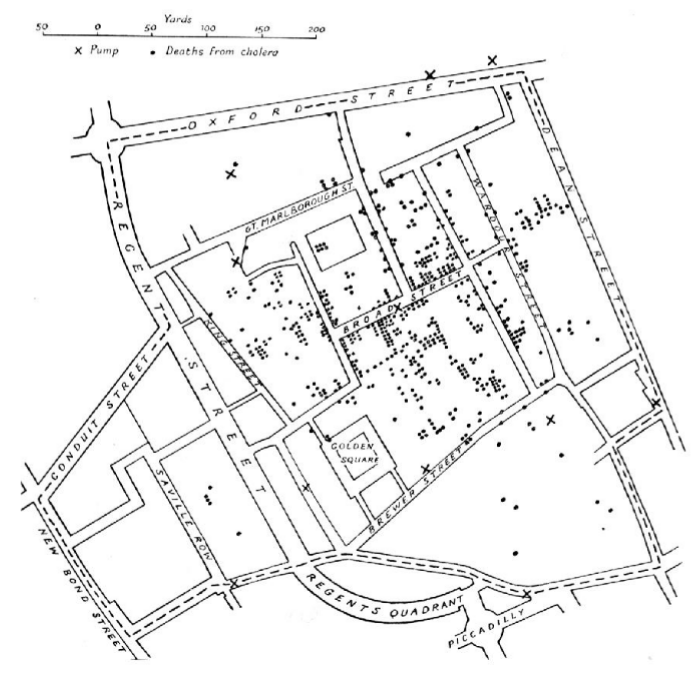
\includegraphics[width=\textwidth/4]{1.png}

\section{Geographical Information
Systems (GIS)}
\subsection{Data Models}
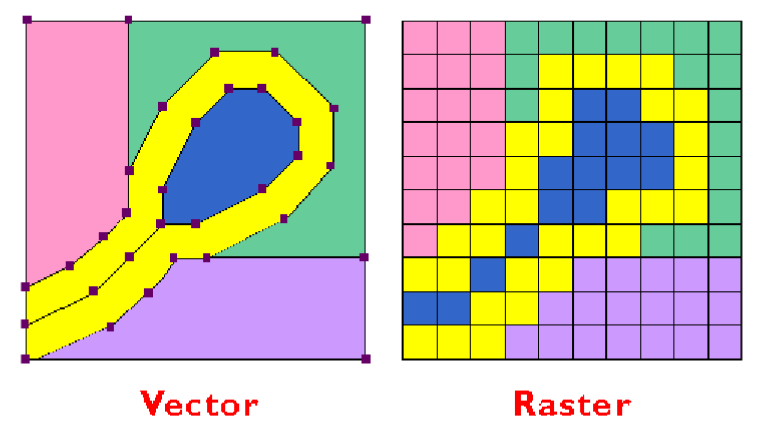
\includegraphics[width=\textwidth/2]{2.png}

hard to go from raster to vector, but easy to go from vector to raster.

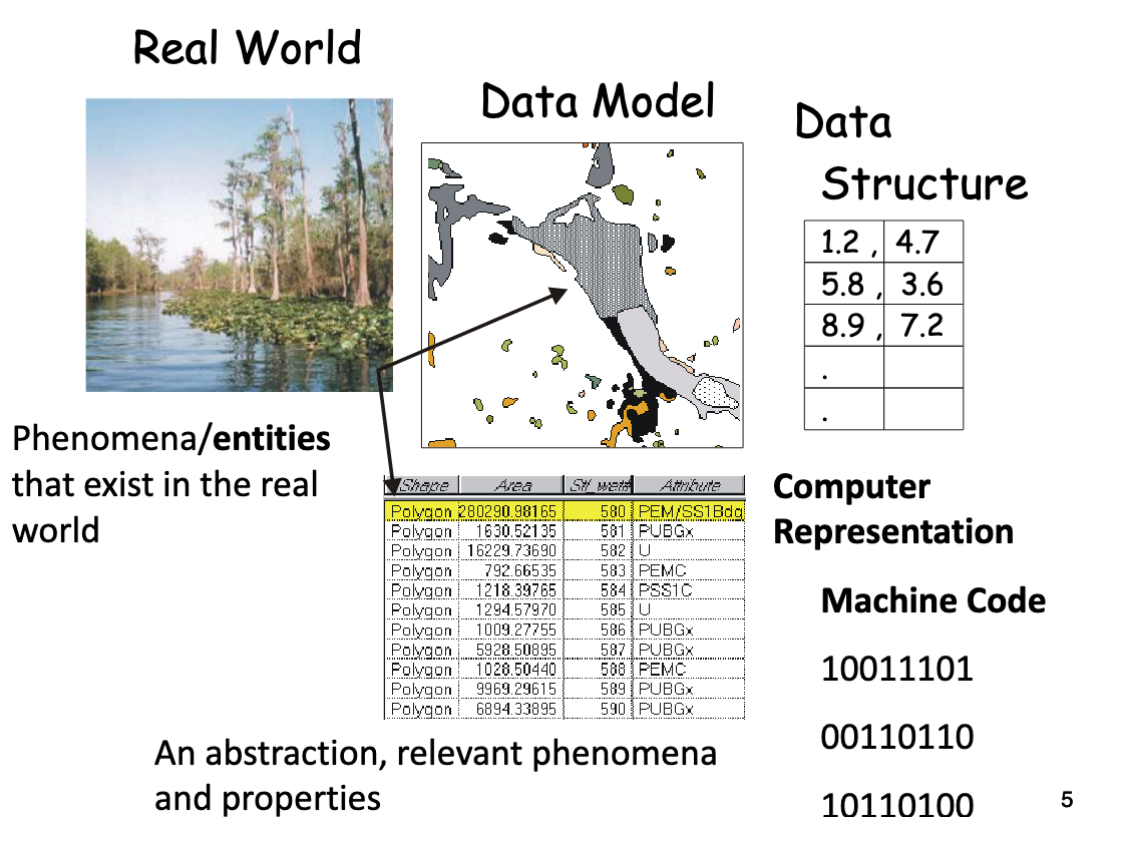
\includegraphics[width=\textwidth/2]{3.png}

GIS and knowledge graphs are difficult to test, expect coding questions rather than conceptual.

\subsection{Data Model}
Objects in a spatial
database.

The spatial data
model provides a
formal means of
representing and
manipulating
spatially-referenced
information.

\subsection{Coordinates}
Coordinates are used to define the
location and extent of spatial objects.

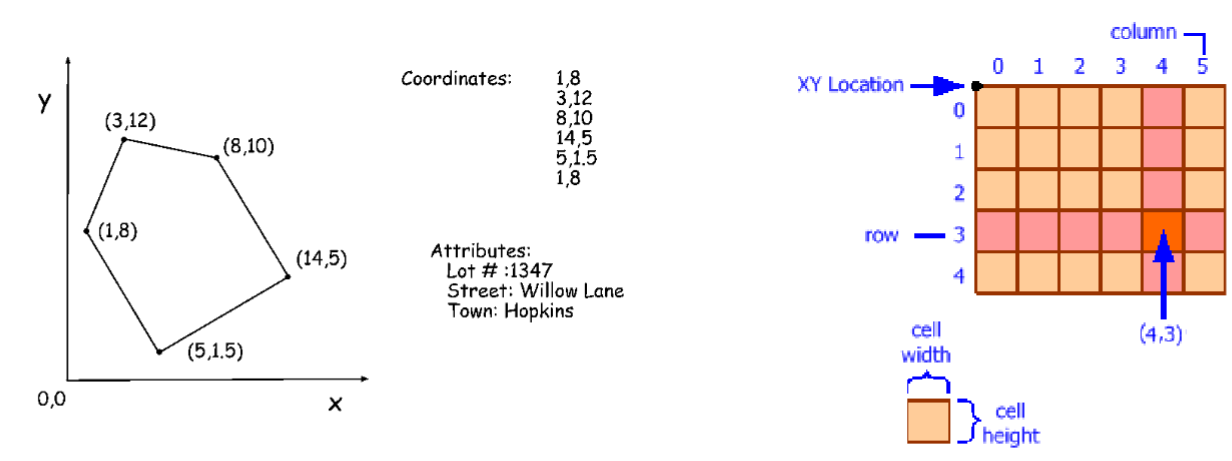
\includegraphics[width=\textwidth/2]{4.png}

\subsection{Attributes}
Attributes describe the spatial object.
Attribute data complements the coordinate
data to define the spatial object.

% 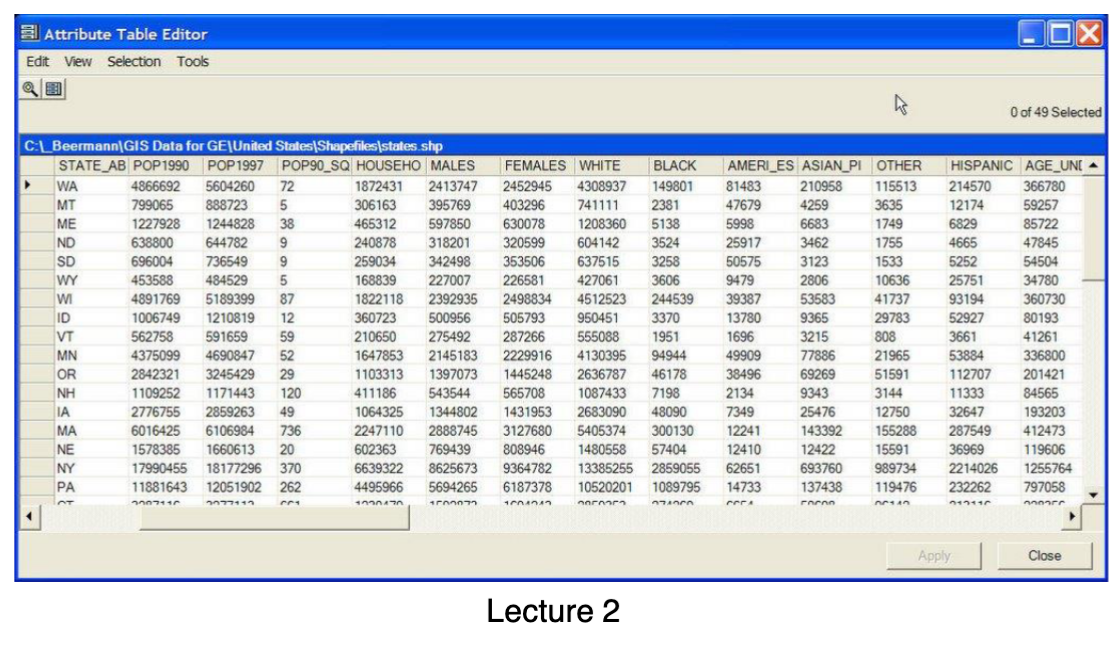
\includegraphics[width=\textwidth]{5.png}

\subsection{Thematic Layers}
\begin{itemize}
    \item A logical separation of data according to theme.
    \item Each layer reflects a particular use or characteristic.
    \item Overlays.
\end{itemize}

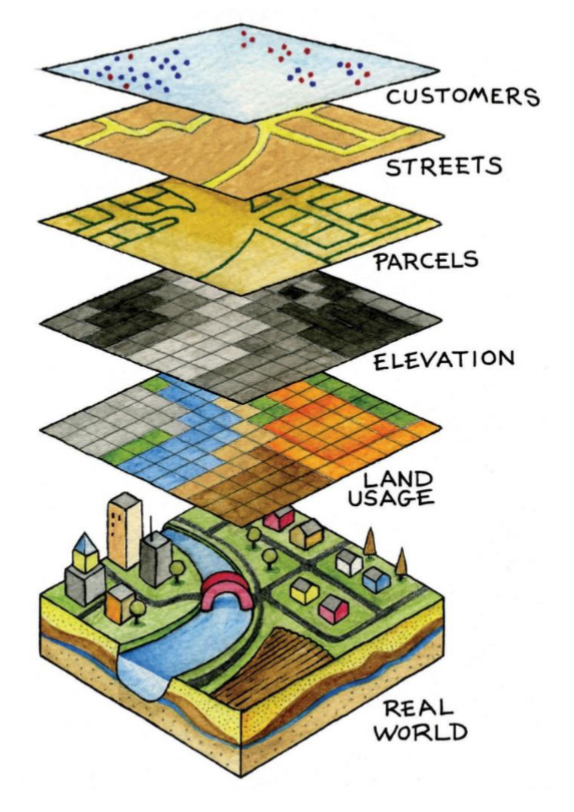
\includegraphics[width=\textwidth/4]{6.png}

\subsection{Coordinate Data}
\begin{itemize}
    \item Latitude \& Longitude
    \begin{itemize}
        \item Origin (intersection of the
        Equator and Greenwich
        meridian)
    \end{itemize}
    \item Spherical Coordinates
    \begin{itemize}
        \item Deg., min., sec. (DMS)
        \item Decimal degrees (DD)
    \end{itemize}
\end{itemize}

\subsection{The Earth is not a Sphere}
\begin{itemize}
    \item It’s close to an Oblate Spheroid. Why?
    \item But there are height variations
    \begin{itemize}
        \item Not just mountains, also density anomalies
    \end{itemize}
\end{itemize}

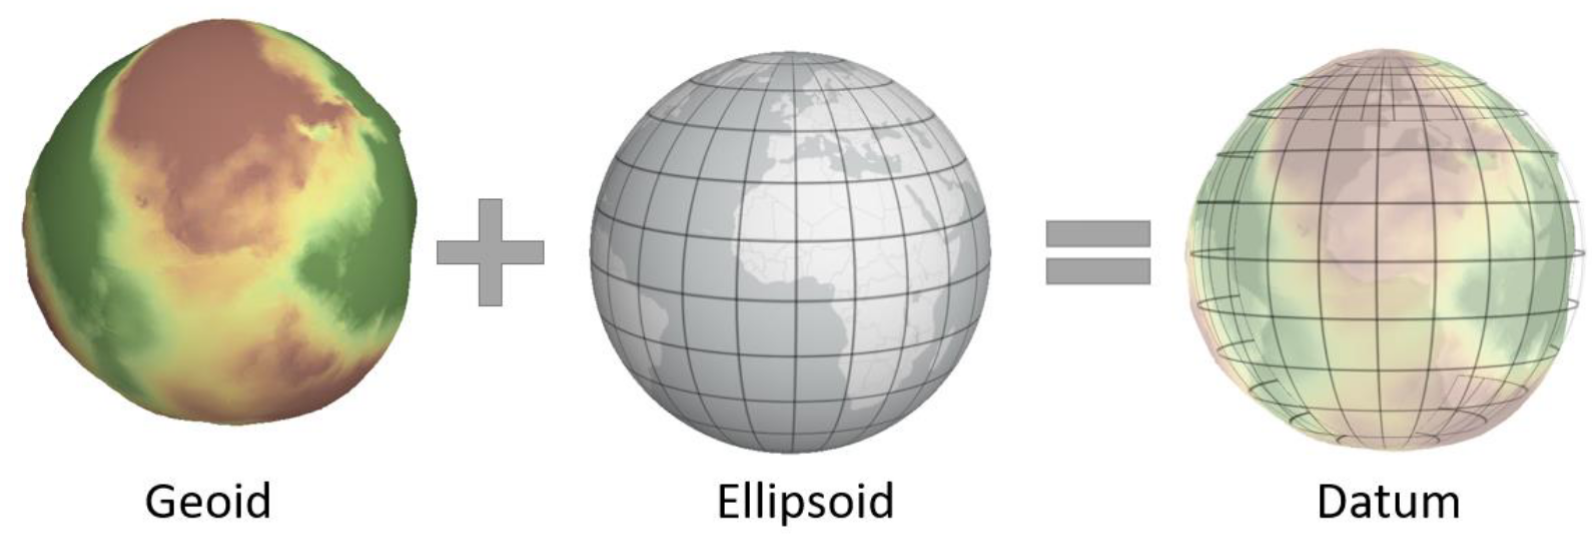
\includegraphics[width=\textwidth/2]{7.png}

\subsection{Ellipsoid}
\begin{itemize}
    \item The Earth is best approximated by an ellipsoid
    \item Ellipsoid is defined by:
    \begin{itemize}
        \item Semi-major axis (a)
        \item Semi-minor axis (b)
        \item Flattening (f) = (a-b)/a
    \end{itemize}
\end{itemize}

\subsection{Geographic vs. Projected
Coordinate System and Raster Coordinate Reference Systems}
\begin{itemize}
    \item Geographic Coordinate
    System (GCS)
    \begin{itemize}
        \item Spheroidal
        approximation of Earth’s
        surface
    \end{itemize}
    \item Projected Coordinate
    System (PCS)
    \begin{itemize}
        \item Projection of GCS onto
        rectangular (Euclidean)
        map coordinates for
        viewing
    \end{itemize}
    \item Raster Coordinate Reference System
    \begin{itemize}
        \item for warping 2D imaging to a CRS
    \end{itemize}
\end{itemize}

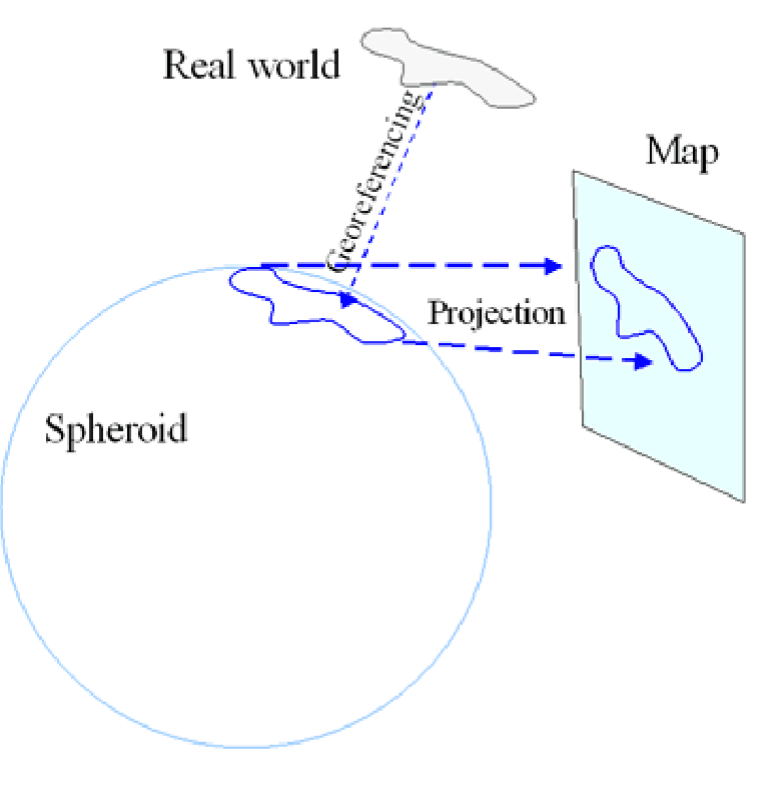
\includegraphics[width=\textwidth/4]{8.png}

\subsection{Nomenclature of Geographic
Coordinate System}
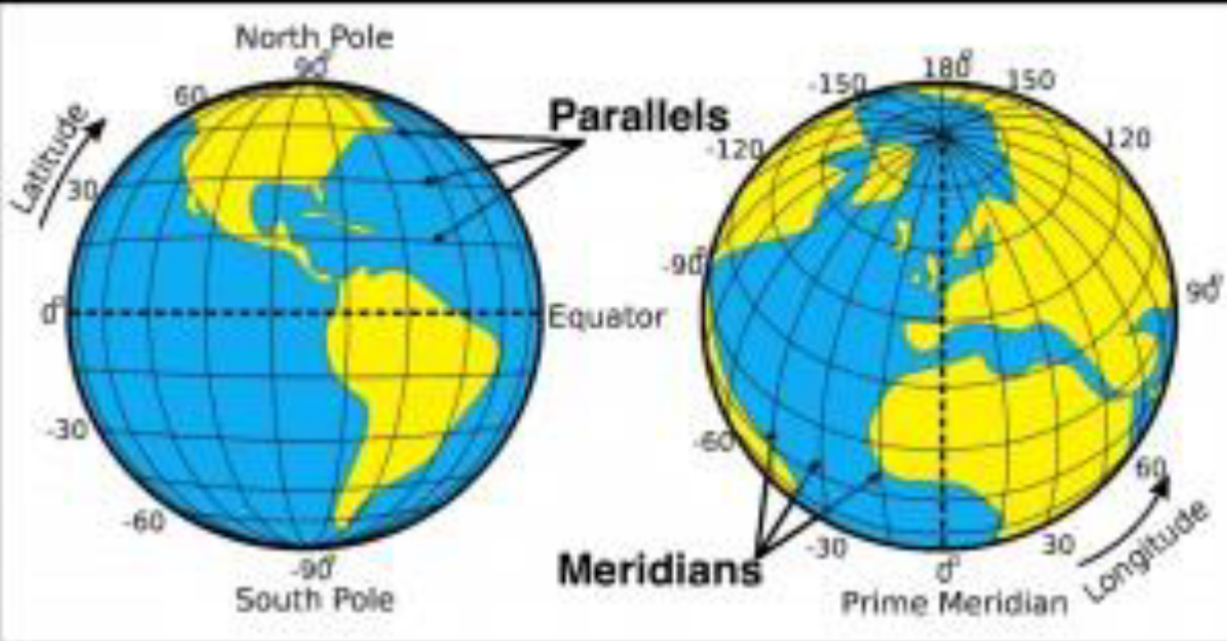
\includegraphics[width=\textwidth/2]{9.png}

\subsection{Properties of Projected
Coordinate Systems (PCSs)}
Three main
types of
projections:
\begin{itemize}
    \item [a] Cylindrical
    \item [b] Conical
    \item [c] Planar
\end{itemize}

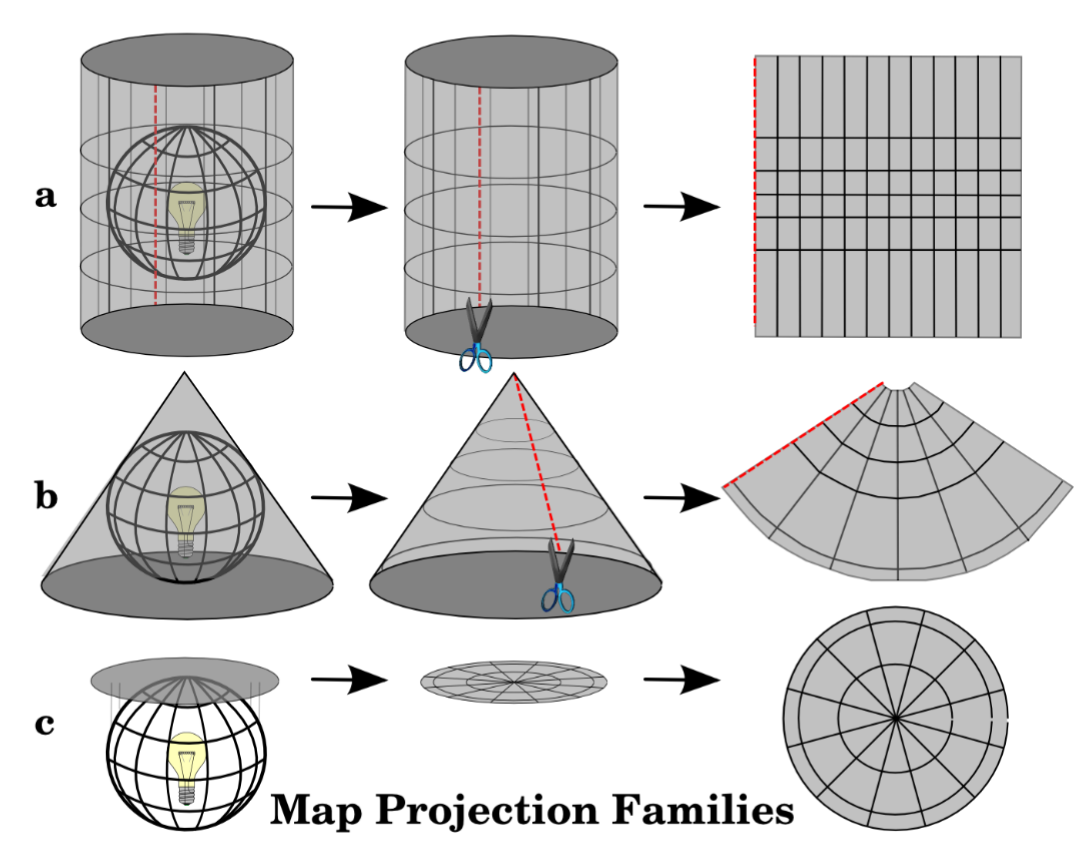
\includegraphics[width=\textwidth/2]{10.png}

\subsection{Projected Coordinate Systems}

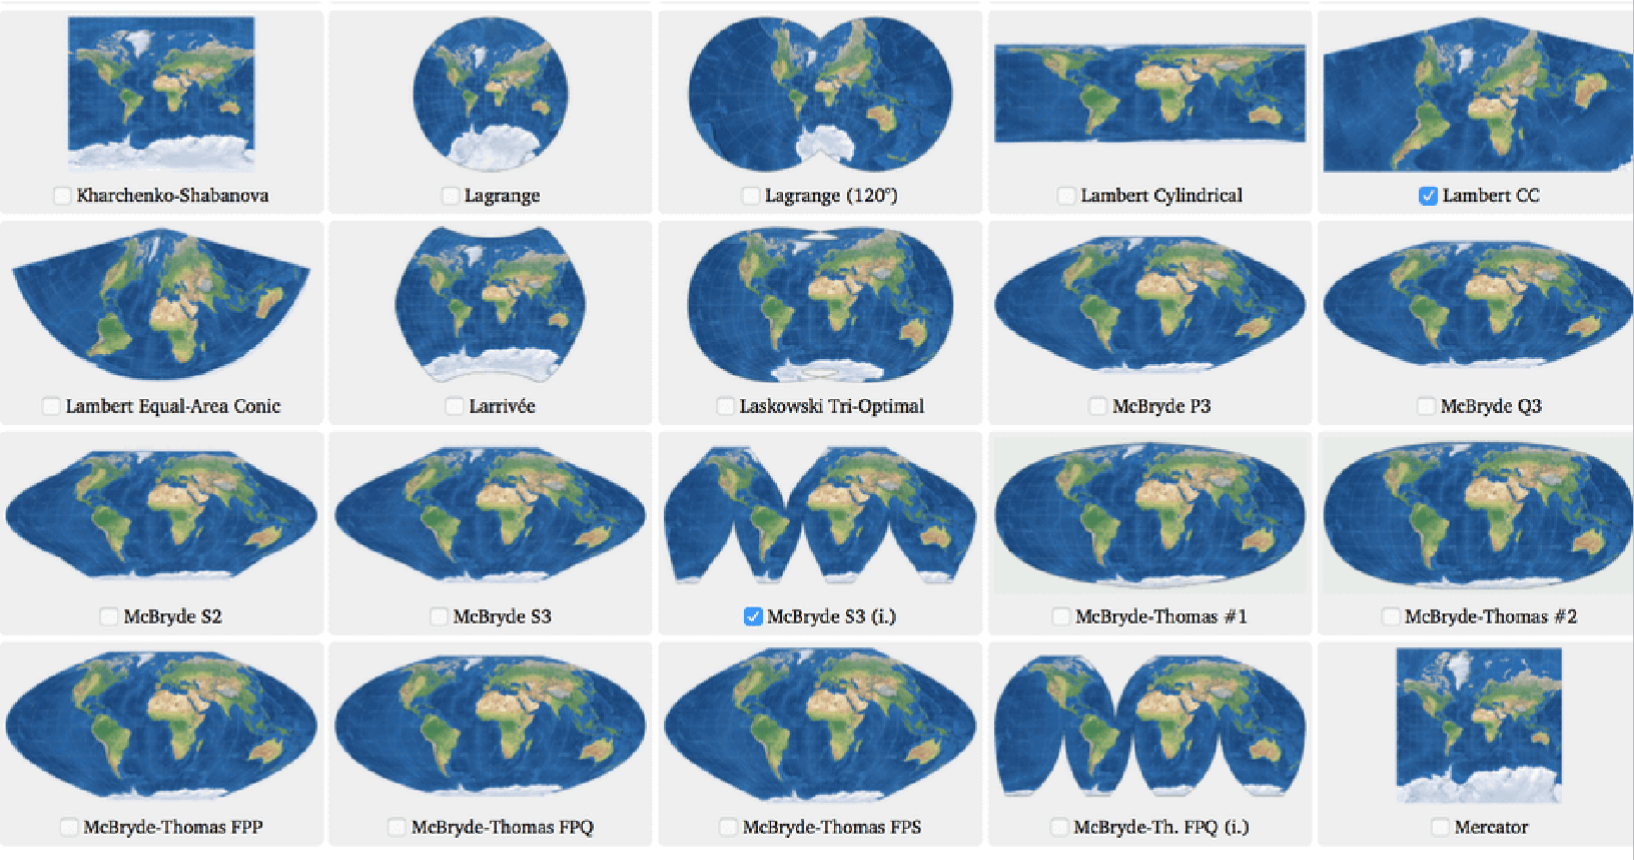
\includegraphics[width=\textwidth/2]{11.png}

\subsection{Properties of PCSs}
\begin{itemize}
    \item Why so many PCSs?
    \item Different PCSs maintain different spatial
    properties
    \begin{itemize}
        \item NESW Cardinal Directions
        \item Angles
        \item Surface Area of Different Regions
        \item Distances between points
    \end{itemize}
\end{itemize}

\subsection{Conversion from Spherical to
Cartesian}

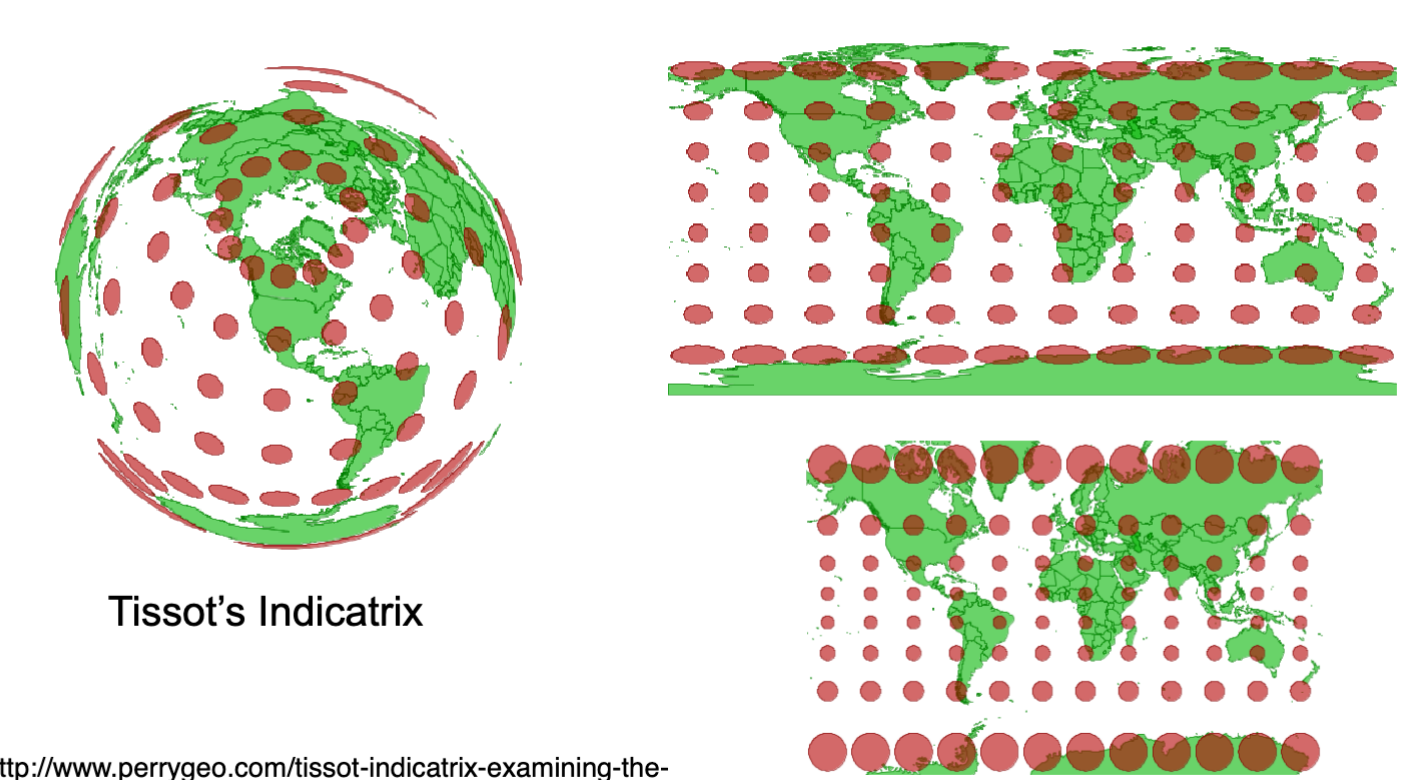
\includegraphics[width=\textwidth/2]{12.png}

\subsection{Converting Arc to Surface
Distance}
At the equator, one degree
of longitude is about 111km

not tested on euclidean to spherical conversion

\begin{equation}
    d = r \cdot \theta
\end{equation}

Where d is the ground distance, r is the
radius of the sphere and the angle is
specified in radians, 360 degrees = 2 $\pi$ radians.

\subsection{Great Circle}
A great circle is defined as any line resulting from a
plane passing through the center of the globe

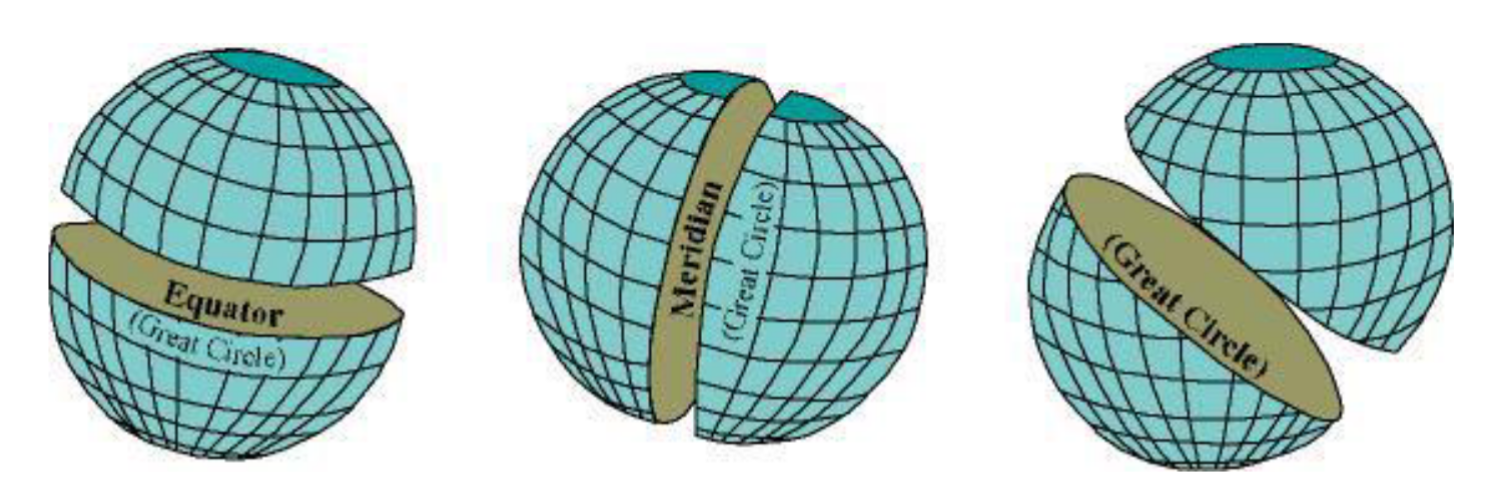
\includegraphics[width=\textwidth/2]{13.png}

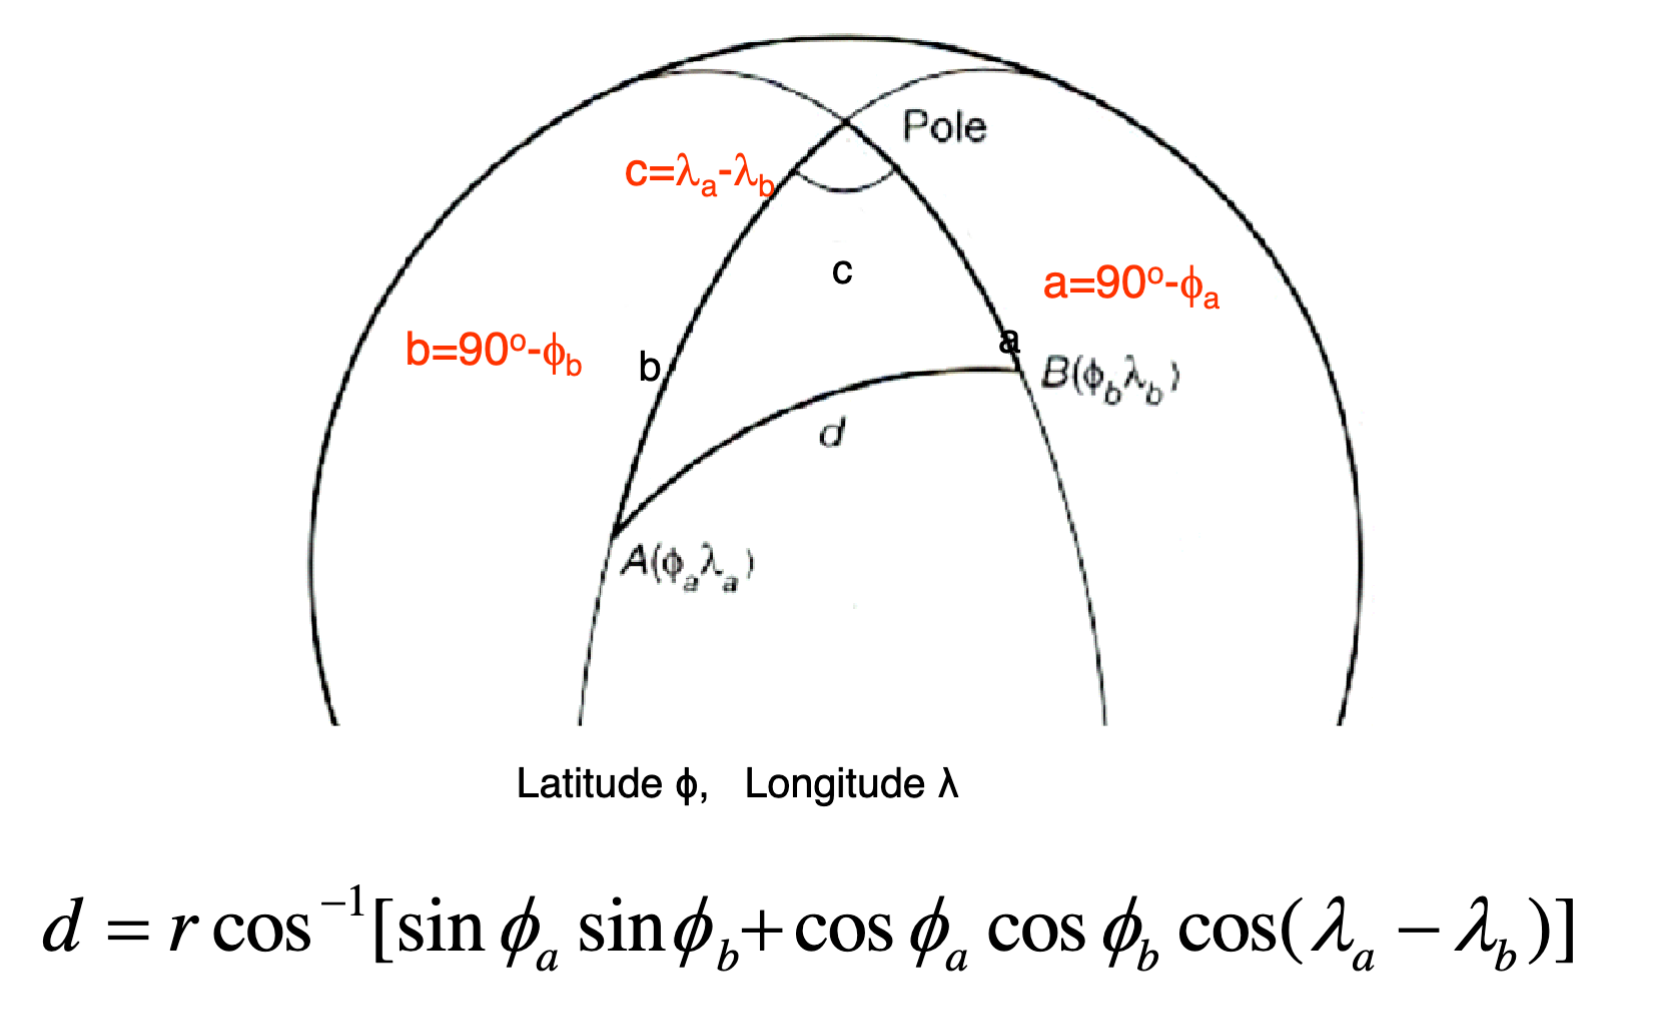
\includegraphics[width=\textwidth/2]{14.png}

\subsection{Conversion from Geographic to
Cartesian Coordinates}
\begin{equation}
    x = r \cdot \cos(\phi) \cdot \cos(\lambda)
\end{equation}
\begin{equation}
    y = r \cdot \cos(\phi) \cdot \sin(\lambda)
\end{equation}
\begin{equation}
    z = r \cdot \sin(\phi)
\end{equation}

This formula requires latitude and longitude to be in radians.

\subsection{Common GIS Data Models}
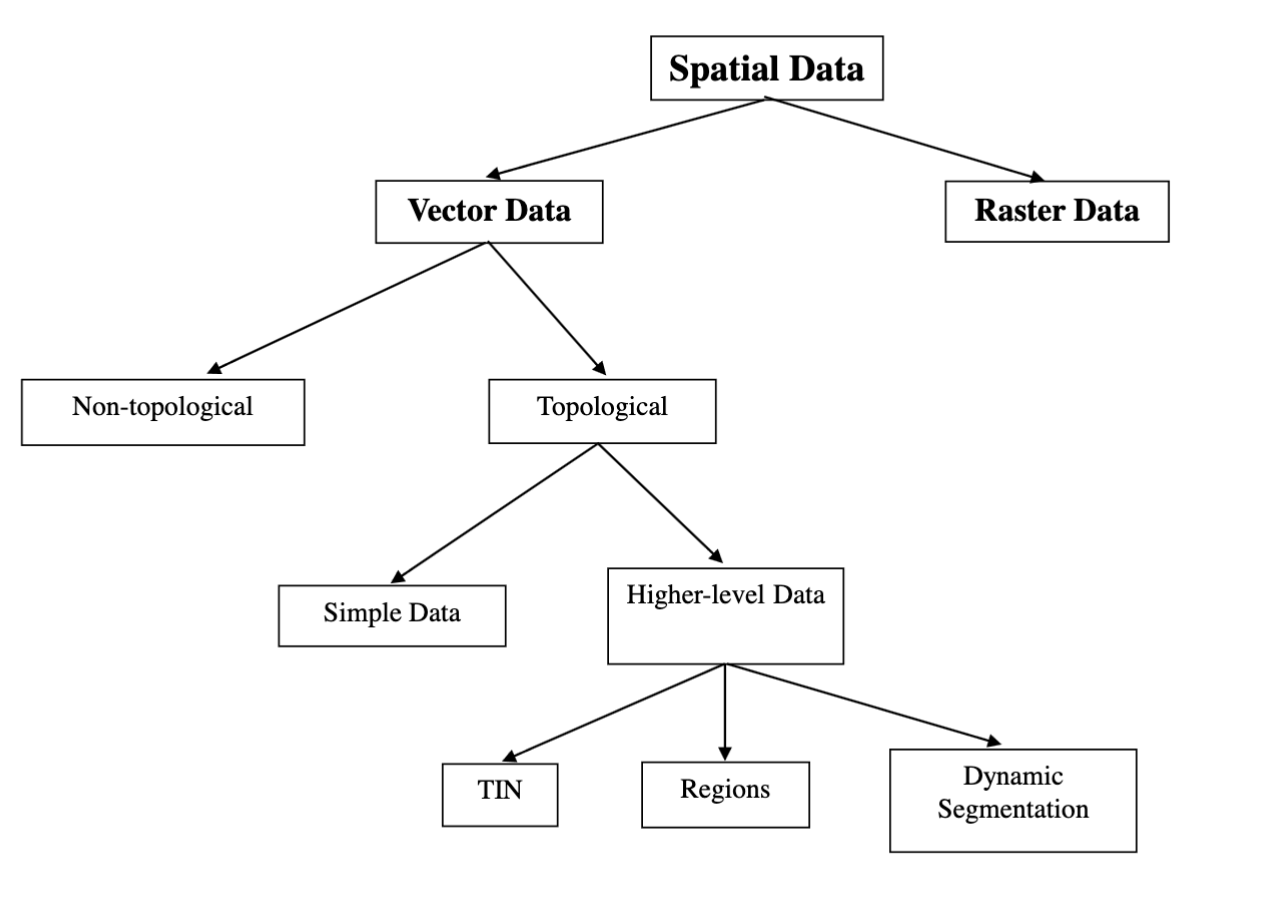
\includegraphics[width=\textwidth/2]{15.png}

\subsection{Two Most Common
Spatial Data Models}

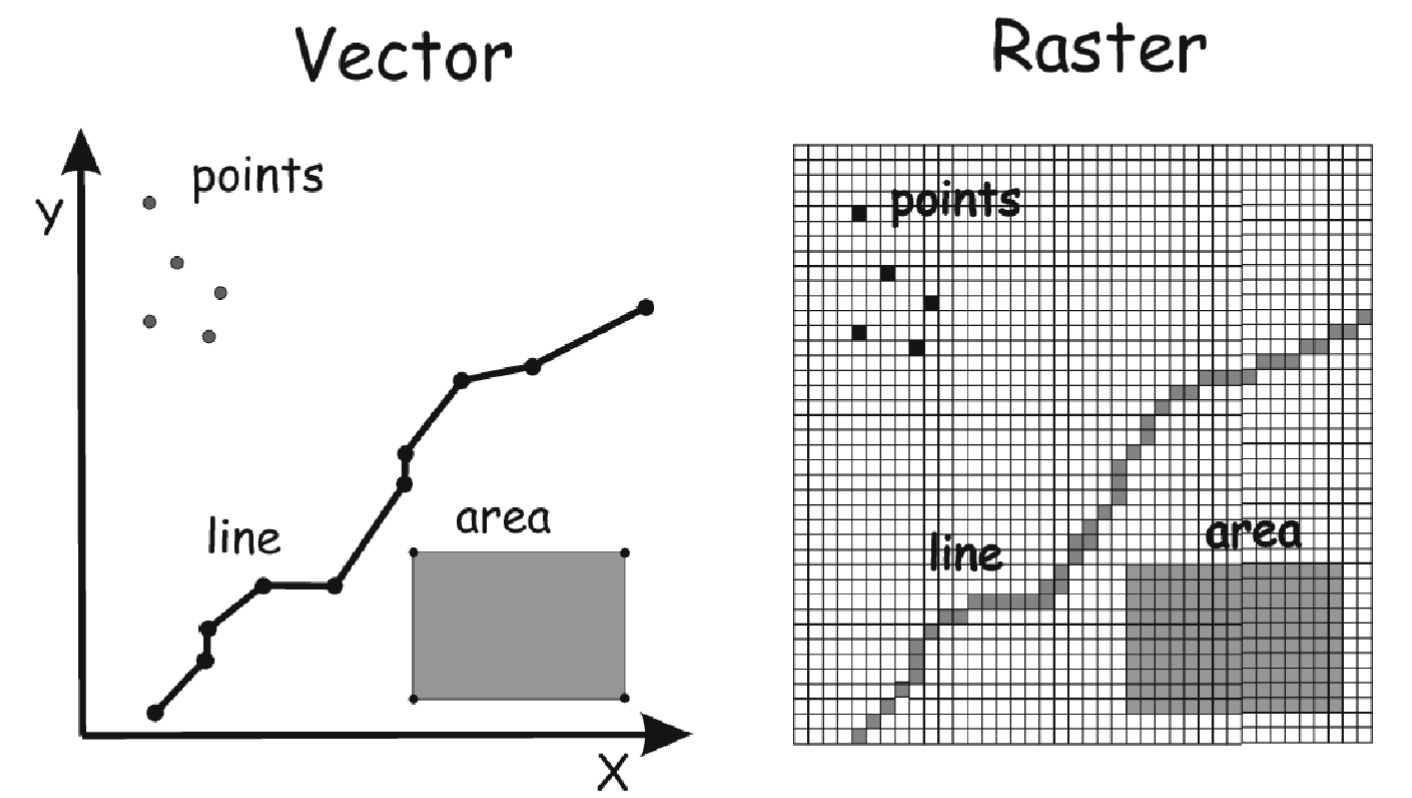
\includegraphics[width=\textwidth/3]{16.png}

\subsection{Triangulated Irregular Network
(TIN)}

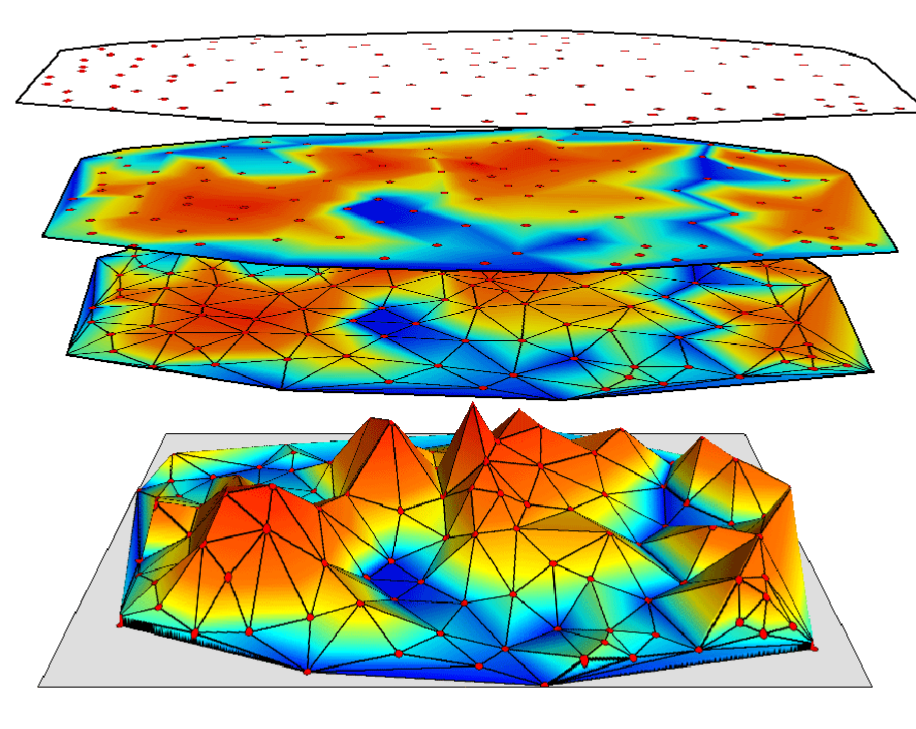
\includegraphics[width=\textwidth/3]{17.png}

\subsection{Regions}
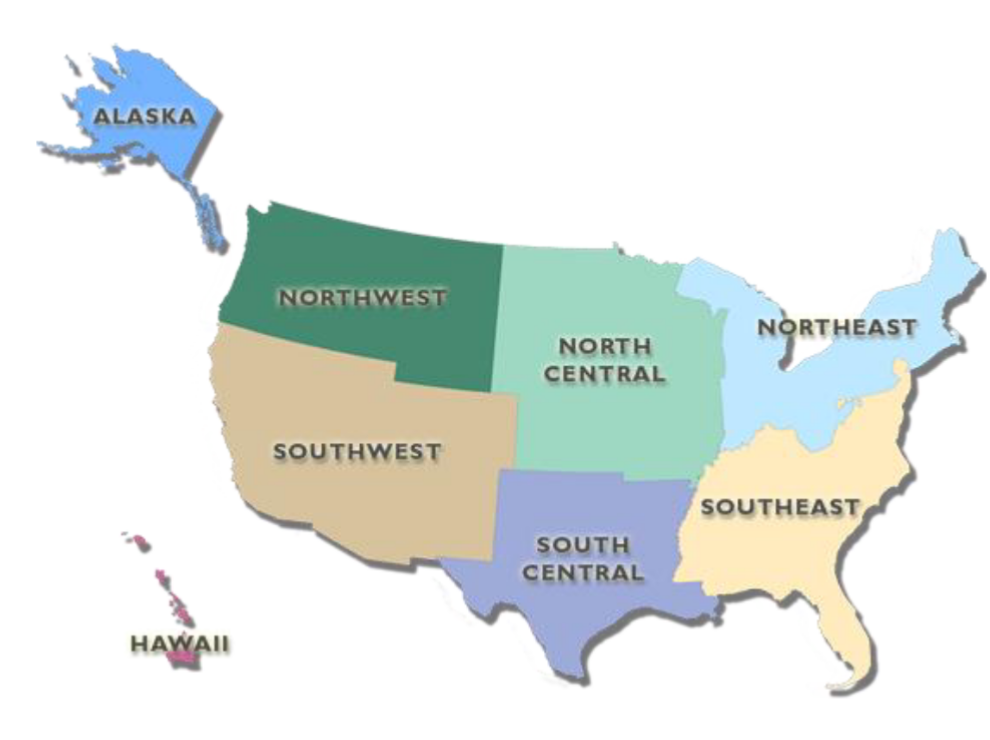
\includegraphics[width=\textwidth/3]{18.png}

\subsection{Contour Lines over a Raster}
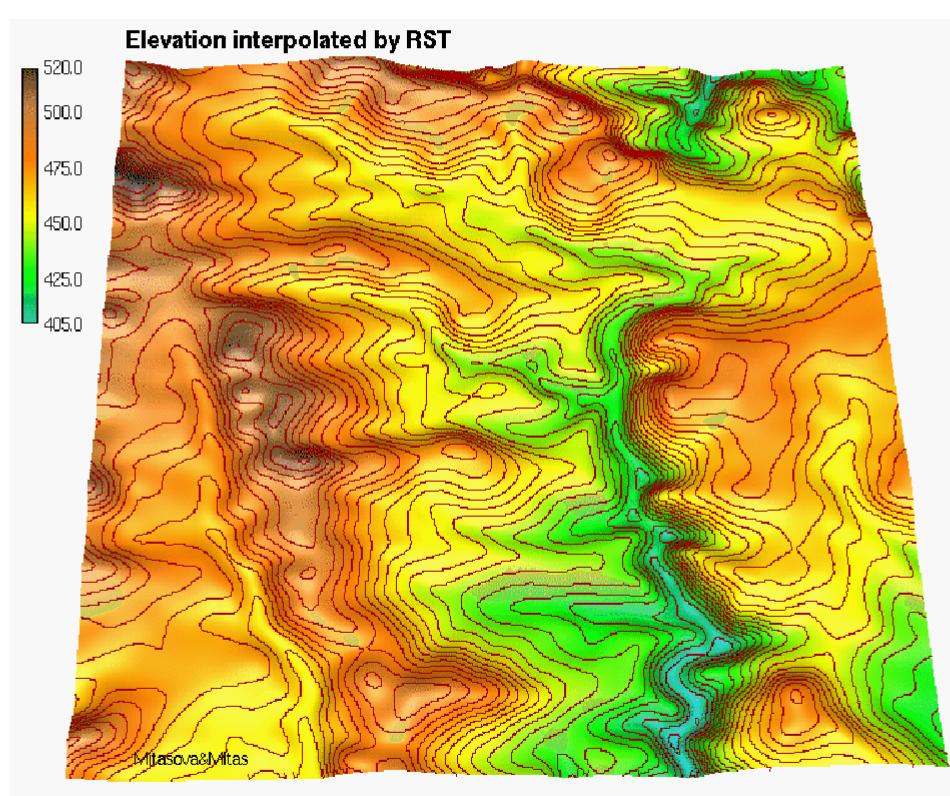
\includegraphics[width=\textwidth/2]{19.png}

\subsection{Vector \& Raster}
\begin{itemize}
    \item Vector is better at representing discrete
    features. (objects, roads, buildings)
    \item Raster is better at representing continuous
    features (imaging, elevation, temperature)
    \item A project may contain both vector and
    raster layers.
    \item Spatial operations can only be performed
    on one type of layer.
    \item The best data model for a given layer
    depends upon the operations, the
    experience and the views of the user.
    \item No decision is final, as one can be
    converted to the other.
\end{itemize}

\subsection{Vector Terminology}
\begin{itemize}
    \item The terms
    polygon / area /
    shape will be
    used
    interchangeably.
    \item A polyline is one
    or more
    connected lines.
    \item A polygon is a
    polyline that
    starts at ends at
    same point.
\end{itemize}

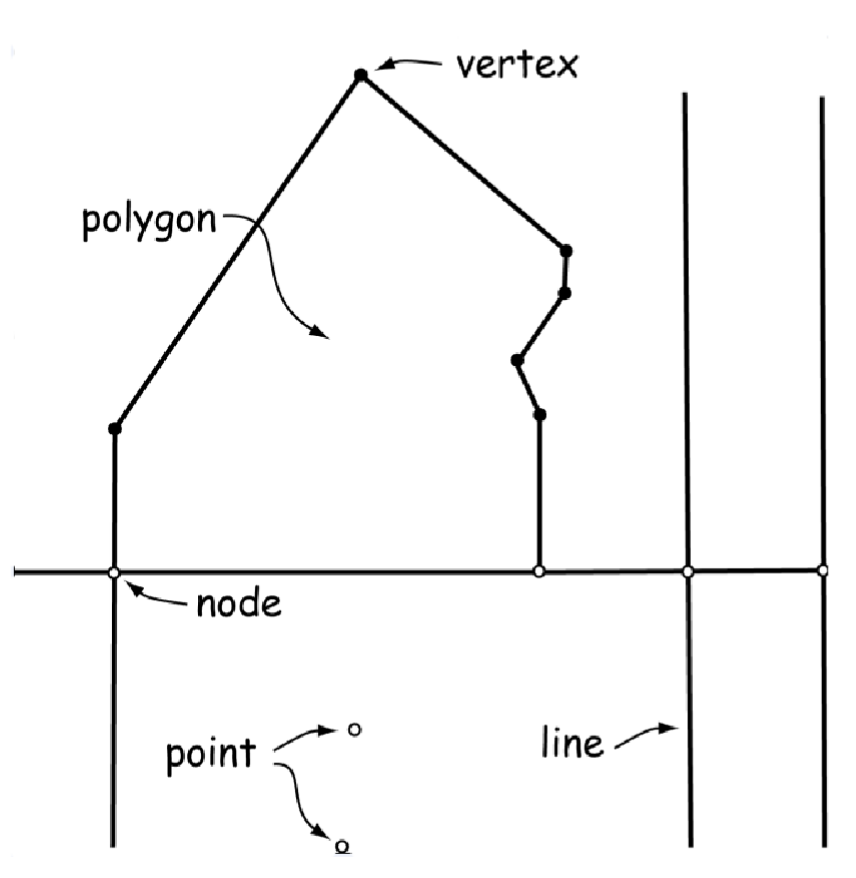
\includegraphics[width=\textwidth/3]{20.png}

\subsection{Multiple Representations}
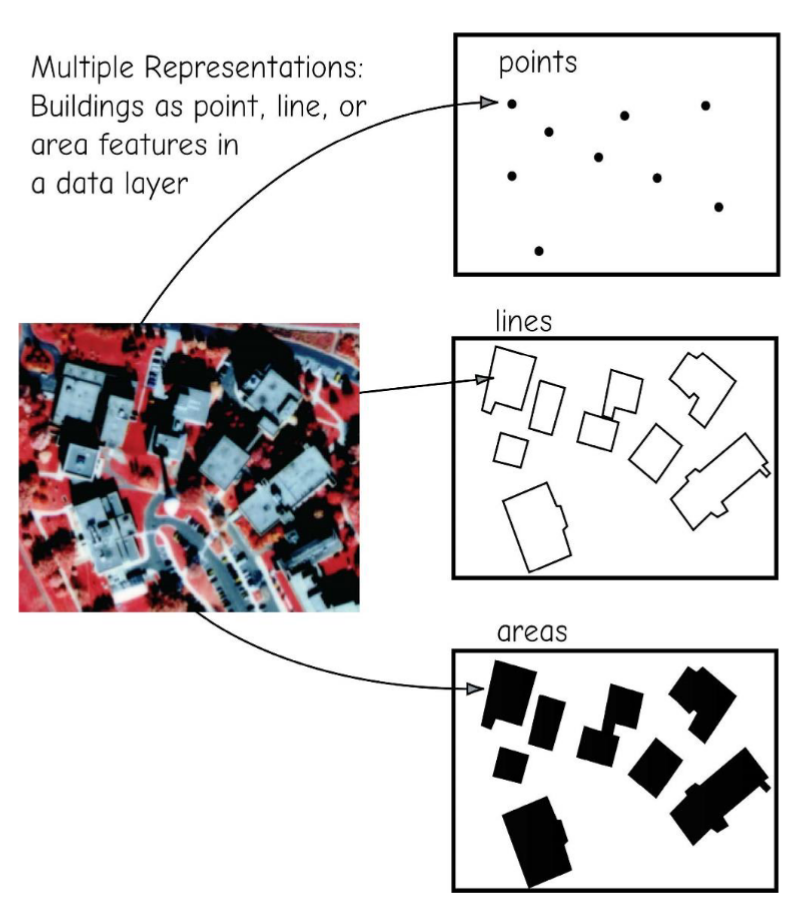
\includegraphics[width=\textwidth/3]{21.png}

\subsection{Vector Model}
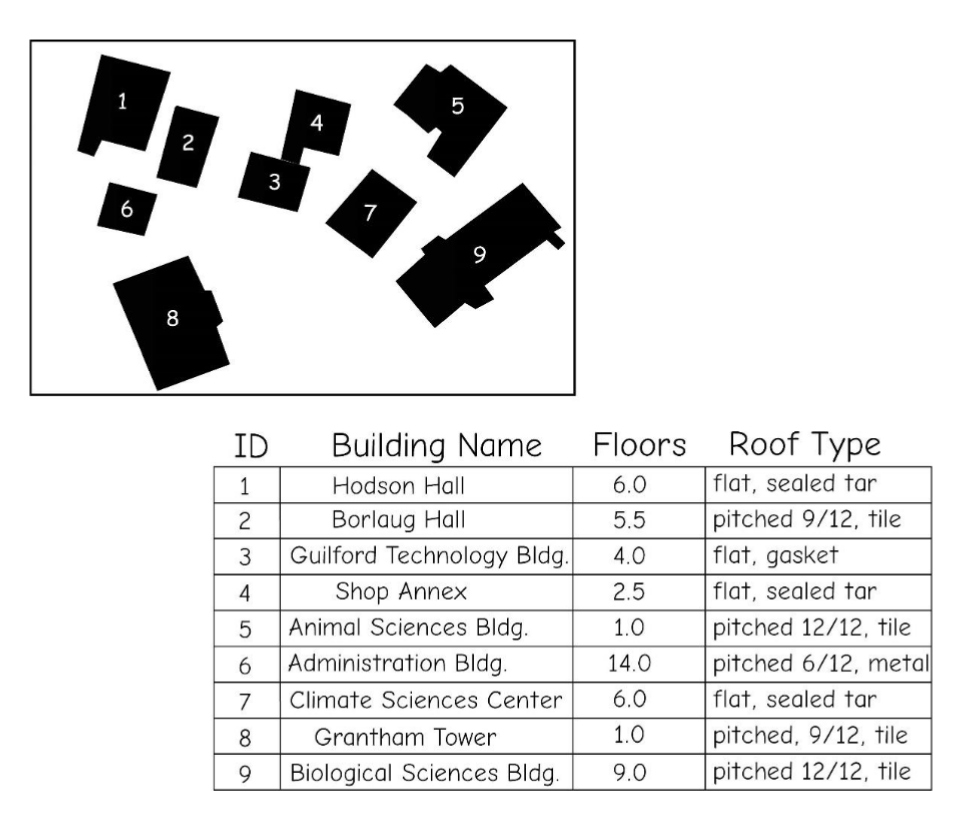
\includegraphics[width=\textwidth/3]{22.png}

\subsection{Single Part Features}
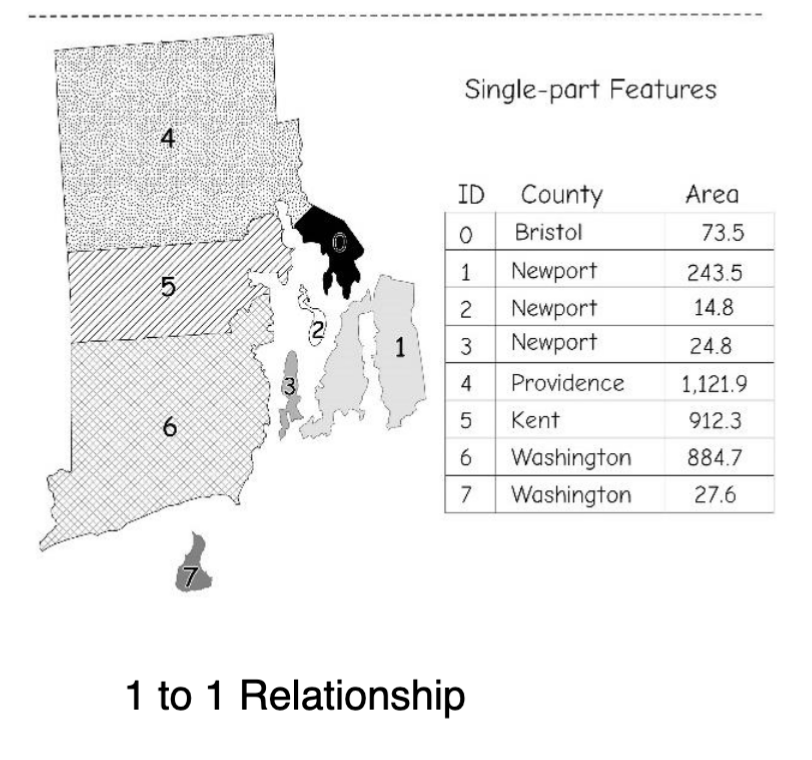
\includegraphics[width=\textwidth/3]{23.png}

\subsection{Multipart Features}
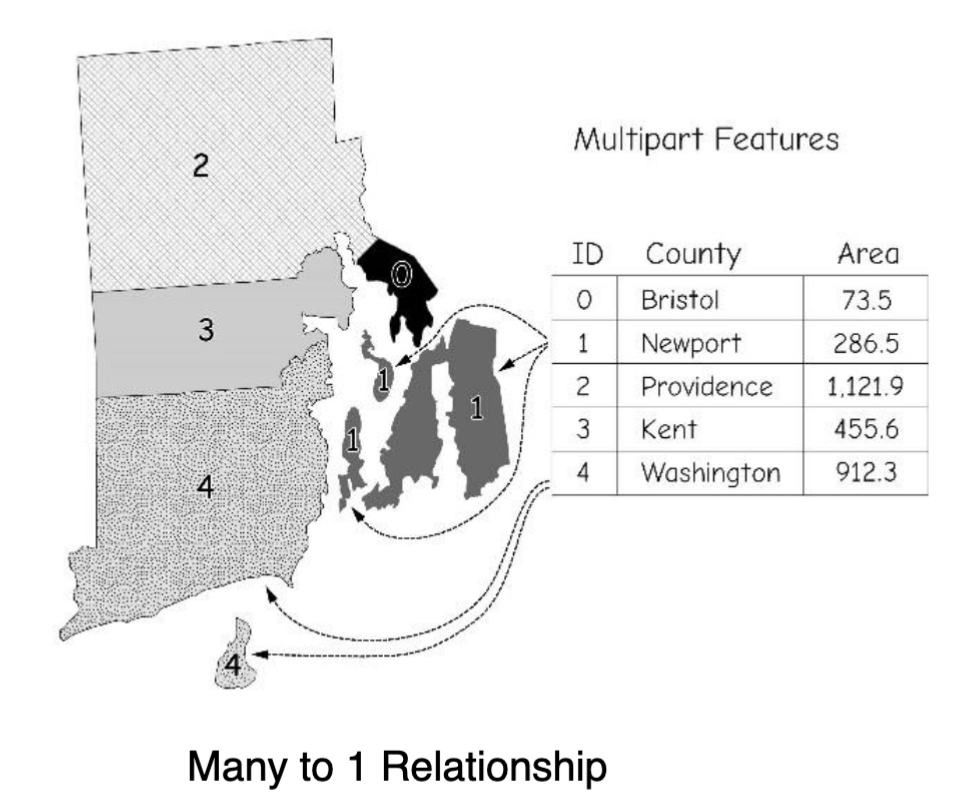
\includegraphics[width=\textwidth/3]{24.png}

\subsection{Multipart to Single-Part Problem}
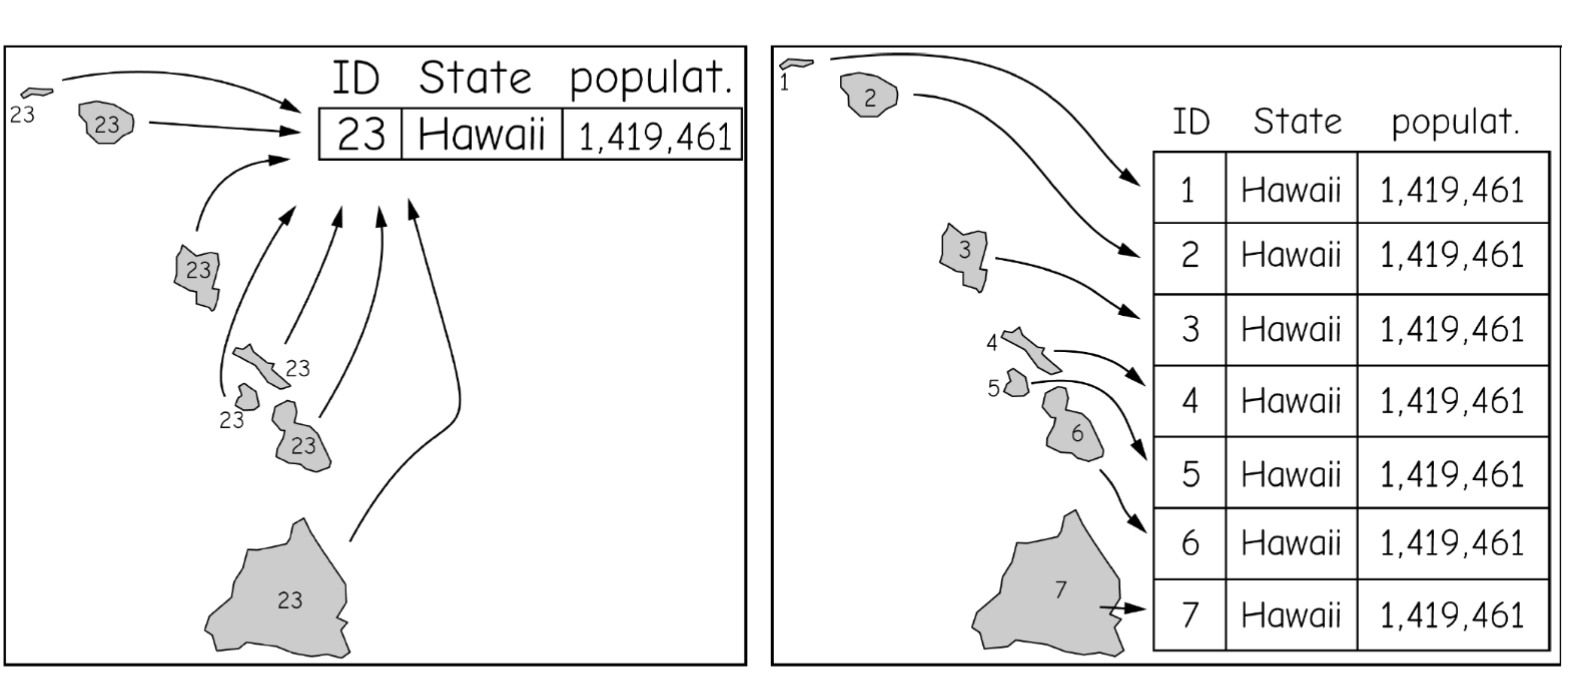
\includegraphics[width=\textwidth/3]{25.png}

\subsection{Polygon Inclusion}
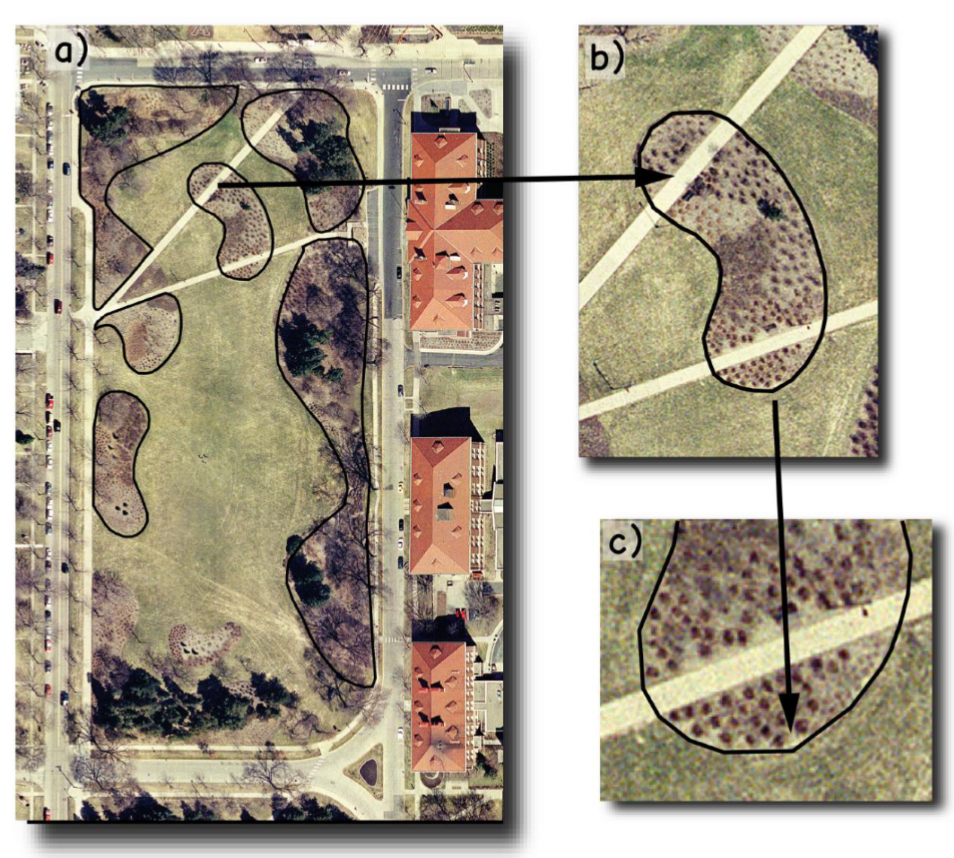
\includegraphics[width=\textwidth/3]{26.png}

\subsection{Polygon Inclusions}
\begin{itemize}
    \item Areas in polygons that are part of the
    polygon, but different from the rest of the
    polygon: e.g. Islands in a lake
    \item Solutions:
    \begin{itemize}
        \item Create separate polygons for each inclusion.
        \item Create an attribute column for coding
        inclusions.
    \end{itemize}
\end{itemize}

\subsection{Key Ideas to Understand}
\begin{itemize}
    \item GIS data consists of layers
    \item Layers can either be Raster or Vector
    \item Each layer has a coordinate reference system
    (CRS)
    \begin{itemize}
        \item Geographic Coordinate System (GCS)
        \begin{itemize}
            \item Spherical coordinates on approximation of Earth’s surface
        \end{itemize}
        \item Projected Coordinate System (PCS)
        \begin{itemize}
            \item Euclidean coordinates for projection onto a rectangular map
            for viewing
            \item Different PCS’s maintain different properties
        \end{itemize} 
    \end{itemize}
\end{itemize}

exam: likely 1 high level question maybe 2

\end{document}